

\pdfoutput=1

\documentclass[envcountsame]{llncs}

\usepackage[utf8]{inputenc}

\usepackage[protrusion=true,expansion=true]{microtype}


\usepackage[style=numeric,
%  backref=true,
 isbn=false,
 maxnames=3,
 maxbibnames=99 ,                
 uniquename=init ,
]{biblatex}
\bibliography{literature.bib}

\usepackage{ownstylesansthm}

\usepackage{comment}
\excludecomment{Long}\includecomment{Short}
% \includecomment{Long}\excludecomment{Short}

\pagestyle{plain}

\begin{document}

\title{Coinductive data types\\in intensional Martin-L\"of type theory}

\author{Benedikt Ahrens and R\'egis Spadotti}

\institute{
Institut de Recherche en Informatique de Toulouse\\
Universit\'e Paul Sabatier, 
Toulouse}

\newcommand{\fat}[1]{\textbf{#1}}





\maketitle

% \tableofcontents

\begin{abstract}


 In this work, we study the notions of \emph{relative comonad} and \emph{comodule over a relative comonad}, and  
 use these notions to give a terminal coalgebra semantics for the coinductive type families of streams and
 of infinite triangular matrices, respectively, in intensional Martin-L\"of type theory.
 Our results are mechanized in the proof assistant \coq.
   
  
  \end{abstract}




 


\section{Preliminaries}\label{sec:preliminaries}

In this section we present some particular categories and functors used later on, and fix some notation.


\begin{definition}[Some categories]\label{def:set_setoid}
 We denote by $\Set$ the category of types (of a fixed universe) and total functions between them in Martin-L\"of type theory. 
 A morphism $f$ in this category is denoted by $f : A \to B$.
 
 We denote by $\Setoid$ the category an object of which is a \emph{setoid}, i.e.\ a type equipped with an equivalence relation.
 A morphism between setoids is a type-theoretic function between the underlying types that is compatible in the obvious sense with the equivalence relations of the source and target setoids.
 If $A$ is a setoid, we also use $A$ to refer to its underlying type, and thus write $a:A$ for an element $a$ of the type underlying the setoid $A$. 
 We write $a\sim a'$ for related elements $a$ and $a'$ in $A$.
 We consider two parallel morphisms of setoids $f,g:A\to B$ equal if for any $a:A$ we have $fa \sim ga$.
 
 We also write $f:A\to B$ for a morphism $f$ between objects $A$ and $B$ in some category, in particular in the category of types.
 \end{definition}



\begin{definition}\label{def:eq}
 The functor $\eq : \Set\to\Setoid$ is defined as the left adjoint to the forgetful functor $U : \Setoid \to \Set$.
  Explicitly, the functor $\eq$ sends any type $X$ to the setoid $(X,=_X)$ given by the type $X$ itself, equipped
  with the propositional equality relation $=_X$ specified via Martin-L\"of's identity type on $X$.
\end{definition}


\begin{remark}[Notation for product]
  We denote the category-theoretic binary product of objects $A$ and $B$ of a category $\C$ by $A\times B$.
  We write $\pr_1(A,B) : \C(A\times B, A)$ and $\pr_2(A,B) :\C(A\times B, B)$ for the projections, occasionally omitting the 
  argument $(A,B)$.
  Given $f : \C(A, B)$ and $g : \C(A,C)$, we write $\langle f,g\rangle : \C(A,B\times C)$ for the induced map into the product such that
  $\comp{\langle f,g\rangle}{\pr_1} = f$ and $\comp{\langle f,g\rangle}{\pr_2} = g$.
\end{remark}

Both of the categories of \Cref{def:set_setoid} have binary products; they are \emph{cartesian monoidal}, i.e.\ the terminal 
object is neutral with respect to the product. Functors preserving the monoidal structure up to isomorphism
are called \emph{strong monoidal}:

\begin{definition}\label{def:monoidal_functor}
 A functor $F:\C\to\D$ between cartesian monoidal categories is \fat{strong monoidal} if, for any two objects $A$ and $B$ of $\C$,
  the morphism
 \[ \phi^F_{A,B} := \bigl\langle F(\pr_1), F(\pr_2) \bigr\rangle : \D\bigl(F(A\times B), FA\times FB\bigr)\enspace  \] 
 is an isomorphism.
 (Note that for \emph{cartesian} monoidal categories, the family $\phi$ of morphisms automatically 
  is compatible with the unitators and associators of the source and target categories, 
  since it is given by a universal property.)
\end{definition}

\begin{example}
  The functor $\eq: \Set \to \Setoid$ of \Cref{def:eq} is strong monoidal.
\end{example}


\section{Codata types in intensional Martin-L\"of type theory}\label{sec:tri}

We consider two particular coinductive type families in Intensional Martin-L\"of type theory (IMLTT) \parencite{martin_lof}, 
a type-theoretic foundational system.
For $a,b : A$, we denote by $a = b$ the Martin-L\"of identity type between $a$ and $b$.

In this section, we present these types, and we also define \emph{bisimilarity} for each codata type.
Bisimilarity is a coinductively defined equivalence relation on types which is considered 
as the appropriate notion of sameness on inhabitants of these types \parencite{DBLP:conf/types/Coquand93, DBLP:journals/corr/abs-cs-0603119}.
A coinductive type with bisimilarity hence forms a setoid as in \Cref{def:set_setoid}.
We thus denote bisimilar elements using an infix $\sim$, as in $t \sim t'$. 

Maps into a coinductive data type are specified by the observations, i.e.\ the value of the destructors, on the output of those maps.  
The precise rule for specifying maps into the considered coinductive type is given in the respective appendix.
In this text, we use a more convenient syntax, as illustrated in \Cref{eq:tail_sredec}.

The first example is the type of \emph{streams} of elements of a given base type $A$. 
The precise set of rules specifying that type is given in \Cref{stream_rules}.
In the presentation we use the notational convention of \Cref{def:set_setoid}, using the same name for a setoid and its underlying type.
\begin{example}\label{ex_stream}
  Let $A$ be a type. The type $\stream A$ of \emph{streams over $A$} is coinductively defined via the destructors 
  given in \Cref{fig:stream_destructors}.
% 
  \begin{figure}[bt]
  \centering

     \def\extraVskip{3pt}
     \def\proofSkipAmount{\vskip.8ex plus.8ex minus.4ex}
    \AxiomC{$t : \stream A$} %\doubleLine
     \UnaryInfC{$\shead_A~t : A$}
      \DisplayProof
                        \hspace{3ex}
                                       \AxiomC{$t : \stream A$}%\doubleLine
                                       \UnaryInfC{$\stail_A~t : \stream A$}
                                       \DisplayProof%
% 
% 
% \vspace{2ex}
% 
\hspace{3ex}
 \centering
                                            \def\extraVskip{3pt}
     \def\proofSkipAmount{\vskip.8ex plus.8ex minus.4ex}
    \AxiomC{$t \sim t'$} %\doubleLine
     \UnaryInfC{$\shead~t = \shead~t'$}
      \DisplayProof
                        \hspace{3ex}
                                       \AxiomC{$t \sim t'$} %\doubleLine
                                       \UnaryInfC{$ \stail~t \sim \stail~t'$}
                                       \DisplayProof   
%   \end{center}
  \caption{Destructors and bisimilarity for the coinductive family $\stream$} \label{fig:stream_destructors}
\end{figure}
   
   
\end{example}


\begin{Long}

Streams are node-labeled trees where every node has exactly one subtree.
We also consider a type of trees where every node has an arbitrary, but fixed, number of subtrees, 
parametrized by a type $B$.



\begin{example}[Node-labeled trees]\label{ex_trees}
 We denote by $\Tree_B(A)$ the codata type given by one destructor $\shead$ and a family of 
 destructors $(\stail_b)_{b:B}$ with types analogous to those defining $\stream$ of \Cref{ex_stream}.
 We thus obtain $\stream$ by considering, for $B$, the singleton type.
\end{example}

\end{Long}

Another codata type we consider models
\emph{infinite triangular matrices}. It is more sophisticated than the type of streams as one of its destructors is \emph{heterogeneous}:



\begin{example}\label{ex_tri}
This codata type is studied in detail by
 \textcite{DBLP:conf/types/MatthesP11}.
 We give a brief summary, but urge the reader to consult the given reference 
 for an in-depth explanation. 
 The codata type family $\Tri$ of infinite triangular matrices 
 is parametrized by a fixed type $E$ for entries not on the diagonal, 
 and indexed by another, \emph{variable}, type $A$ for entries on 
 the diagonal. 
\begin{Long}
 Schematically, such a matrix looks like in \Cref{fig_tri}.
 \begin{figure}[bt]
 \centering
 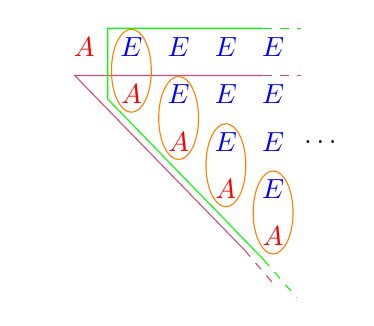
\begin{tikzpicture}[scale = 0.6]
    \foreach \y in {0,...,2}
    {\foreach \x in {\y,...,2}
      \draw (\x+1, -\y) node[color=blue]{$E$} ;
    }
    \foreach \x in {-1,...,3} \draw (\x, -\x-1) node[color=red]{$A$} ;
    \foreach \x in {0,...,3} \draw (\x, -\x)
    node[color=blue]{\textbf{$E$}} ;
    \draw(4,-2) node{$\ldots$};
    
    
      \draw[color=purple!70]  (2.4, -4.3) --node[auto, swap, left]{$\cut$}
     (-1.2,-0.6) -- (2.8,-0.6);
    \draw[color=purple!70, dashed]  (2.8,-0.6) -- (3.6,-0.6);
    \draw[color=purple!70, dashed]  (2.4,-4.3) -- (3.0,-5);

    \draw (-2,0) node{$\head$} ;
    

    \draw[color=green] (2.8,0.4) -- (-0.5,0.4) -- (-0.5, -1.1) --node[auto, swap, left]{$\tail$}
    (2.8,-4.5)  ; 
    \draw[color=green, dashed] (2.8,0.4) -- (3.6,0.4) ; 
    \draw[color=green, dashed] (2.8,-4.5) -- (3.5,-5.3) ; 


    \draw[color=orange](0, -0.5) ellipse (12pt and 25pt) ;  
    \draw[color=orange](1, -1.5) ellipse (12pt and 25pt) ;  
    \draw[color=orange](2, -2.5) ellipse (12pt and 25pt) ;  
    \draw[color=orange](3, -3.5) ellipse (12pt and 25pt) ;  
  \end{tikzpicture}\\[-2ex]
  \caption{An infinite triangular matrix over type $A$ and various operations}\label{fig_tri}
 \end{figure}
\end{Long}
  
 It is specified via two destructors $\head$ and $\tail$, whose types are given in \Cref{fig:tri_destructors}.
\begin{Long}
 Given a matrix over type $A$, its $\tail$---obtained by removing the first element on the diagonal, i.e.\ the $\head$ element---can 
 be considered as a trapezium as indicated by the green line in \Cref{fig_tri}, or alternatively, as
 a triangular matrix over type $E\times A$, by bundling the entries of the diagonal with those above as indicated by the orange frames in \Cref{fig_tri}.
 The latter representation is reflected in the type of the destructor $\tail$.
\end{Long}
\begin{Short}
 Given a matrix over type $A$, its $\tail$---obtained by removing the first element on the diagonal, i.e.\ the $\head$ element---can 
 be considered as a trapezium or, alternatively, as a triangular matrix over type $E\times A$, 
 by bundling the entries of the diagonal with those directly above the diagonal.
\end{Short}

 Bisimilarity on the inhabitants of that type is defined via the destructors of \Cref{fig:tri_destructors}.    
 As with streams, we denote by $\Tri A$ not only the resulting \emph{setoid} of triangular matrices over $A$, but also its
 underlying \emph{type}. 

\begin{figure}[bt]
  \centering

     \def\extraVskip{3pt}
     \def\proofSkipAmount{\vskip.8ex plus.8ex minus.4ex}
    \AxiomC{$t : \Tri~A$} %\doubleLine
     \UnaryInfC{$\head_A~t : A$}
      \DisplayProof
                        \hspace{3ex}
                                       \AxiomC{$t : \Tri~A$}%\doubleLine
                                       \UnaryInfC{$\tail_A~t : \Tri(E\times A)$}
                                       \DisplayProof%
% 
% 
% \vspace{2ex}
% 
 \hspace{3ex}
                                            \def\extraVskip{3pt}
     \def\proofSkipAmount{\vskip.8ex plus.8ex minus.4ex}
    \AxiomC{$t \sim t'$}%\doubleLine
     \UnaryInfC{$\head~t = \head~t'$}
      \DisplayProof
                        \hspace{3ex}
                                       \AxiomC{$t \sim t'$}%\doubleLine
                                       \UnaryInfC{$ \tail~t \sim \tail~t'$}
                                       \DisplayProof   

  \caption{Destructors and bisimilarity for the coinductive family $\Tri$} \label{fig:tri_destructors}
\end{figure}
\end{example}
% 
% 
 

\section{Terminality for streams and infinite triangular matrices}\label{sec:coalgebras_for_tri}

In this section, we define a notion of \enquote{coalgebra} for the signatures of streams and triangular matrices,
respectively. We then show that the codata types $\stream$ and $\Tri$ constitute the terminal object in
the respective category of coalgebras.
We put \enquote{coalgebra} in quotes for the reason that our coalgebras are not defined as coalgebras for a monad or an endofunctor.

The terminal coalgebra result is hardly surprising; however, it is still interesting as it characterizes not only the codata types themselves,
 but also the respective bisimilarity relations and comonadic operations on them, via a universal property.
 


\begin{Long}
\subsection{Coalgebras for $\stream$}

We first consider the homogeneous codata type of streams.
\end{Long}

\begin{definition}%[Coalgebras for $\stream$]
 \label{cat_stream}
  A \fat{coalgebra for $\stream$} is given by a triple $(S,h,t)$ 
  consisting of
  \begin{itemize}
   \item a setoid $S : \Setoid$,
   \item a setoid morphism $h : S \to \eq A$ and
   \item a setoid morphism $t : S \to S$.
  \end{itemize}
  A coalgebra morphism $(S,h,t) \to (S',h',t')$ is given by a setoid morphism $\tau : S \to S'$ such that
     $\comp{\tau}{h} = h'$ pointwise and
     $ \comp{t}{\tau} \sim \comp{\tau}{t'}$ pointwise.
\end{definition}

This defines a category, with the obvious composition and identity. 

\begin{theorem}\label{thm_stream_terminal}
 The following are equivalent:
 \begin{itemize}
  \item the rules given in \Cref{stream_rules};
  \item the category of coalgebras has a terminal object.
 \end{itemize}
\end{theorem}

More precisely, the aforementioned theorem says that the rules given in \Cref{stream_rules} allow to prove that
the category of coalgebras defined in \Cref{cat_stream} has a terminal object.

\begin{example}
  We equip the relative comonad $\Tri$ with the structure of a coalgebra for $\stream$ by defining a 
  morphism of tautological comodules over $\Tri$, given by
   $ t^{\diagonal} := \comp{\tail}{\cut}  : \Tri \to \Tri$.
  The resulting terminal coalgebra morphism
   $(\Tri, t^{\diagonal}) \to (\stream, \stail)$ has as underlying morphism of relative comonads the one defined in \Cref{ex_diag}.
\end{example}

\begin{Long}
 
\begin{remark}
 Fix a type $B$. A result analogous to \Cref{thm_stream_terminal} holds for trees $\Tree_B$ of \Cref{ex_tree_comonad}. 
 We refrain from giving a precise statement of this result.
\end{remark}

\end{Long}

\begin{Long}
\subsection{Coalgebras for $\Tri$}
\end{Long}

In analogy to the definition of coalgebras for the signature of streams, one would define
a coalgebra for the signature of $\Tri$ as a pair $(T,r)$ of a comonad $T$ relative to $\eq : \Set \to \Setoid$ and 
a morphism of comodules $r : T \to T(E\times \_)$. 
It turns out that in this way, one is not capable of obtaining the right auxiliary function $\cut$ for what is
supposed to be the \emph{terminal} such coalgebra (where $\cut$ is used to define the comodule $\Tri(E\times \_)$), namely the pair $(\Tri,\tail)$.
As a remedy, we define a coalgebra to come equipped with a specified operation analogous to $\cut$, and some laws governing
the behavior of that operation:




\begin{definition}%[Relative comonad with cut]
\label{def:rel_comonad_with_cut}
 Let $\C$ and $\D$ be categories with binary products and $F:\C\to\D$ a strong monoidal functor. Let $E:\C_0$ be a fixed object of $\C$.
 We define a \fat{comonad relative to $F$ with cut relative to $E$} to be a comonad $T$ relative to $F$ together with a $\cut$ operation 
    \[ \cut : \forall~A:\C_0, T(E\times A) \to TA \qquad \text{such that}\]
%  satisfying the following axioms:
  \begin{itemize}
%    \item $\forall~A:C_0, \comp{\cut_A}{\counit_A} = \comp{\counit_{E\times A}}{F(\pr_2(E,A))}$;
   \item $\forall~A:C_0, \comp{\cut_A}{\counit_A} = \comp{\lift^T(\pr_2(E,A))}{\counit_{A}}$;
   \item $\forall~A~B:C_0,\forall~f:\D(TA,FB), \comp{\cut_A}{\cobind(f)} = \comp{\cobind(\extend~f)}{\cut_B}$,
  \end{itemize}

  \noindent
  where, for $f:\D(TA,FB)$, we define $\extend(f) : \D\bigl(T(E\times A),F(E\times B)\bigr)$ as
       \[ \extend(f) := \comp{\comp{\langle T(\pr_1) , \cut \rangle}{(\counit_E\times f)}}{{\phi^{F}_{E,B}}^{-1}} \enspace . \]
  
\end{definition}

Morphisms of comonads with cut are morphisms of comonads that are compatible with the respective $\cut$ operations:

\begin{definition}%[Morphism of comonads with cut]
\label{def:morphism_comonad_cut}
 Let $(T,\cut^T)$ and $(S,\cut^S)$ be two comonads relative to a functor $F$ with cut relative to $E$ as in \Cref{def:rel_comonad_with_cut}.
 A \fat{morphism of comonads with cut} is a comonad morphism $\tau$ between the underlying comonads as in \Cref{def:comonad_morphism} that 
 commutes suitably with the respective $\cut$ operations, i.e.\ for any $A : \C_0$,
  $\comp{\tau_{E \times A}}{\cut^S_A}  = \comp{\cut^T_A}{\tau_A}$.
\end{definition}


Comonads with cut relative to a fixed functor $F:\C\to\D$ and $E:\C_0$ form a category $\RComonadWC(F,E)$.
There is the obvious forgetful functor from $\RComonadWC(F,E)$ to $\RComonad(F)$.
Conversely, any comonad $T$ relative to a suitable functor can be equipped with a $\cut$ operation, using functoriality of $T$.
%
\begin{Short}
 Details are given in the long version of this article.
\end{Short}

\begin{Long}
\begin{remark}[Canonical $\cut$ operation]\label{canonical_cut}
 Any comonad $T$ relative to a strong monoidal functor $F:\C\to\D$  can be equipped with a $\cut$ operation relative to 
 $E:\C_0$ satisfying the properties of \Cref{def:rel_comonad_with_cut} by setting
   \[ \ccut_A := \cut_A := \lift^T\bigl(\pr_2(E,A)\bigr) \enspace . \]
 (The extra \enquote{c} of $\ccut$ stands for \enquote{canonical}.)
 It follows from the axioms of comonad morphism that a comonad morphism $\tau : T\to S$ satisfies the equation of \Cref{def:morphism_comonad_cut} 
 for the thus defined operations $\ccut^T$ and $\ccut^S$, hence constitutes a morphism of comonads with cut from $(T,\ccut^T)$ to $(S,\ccut^S)$.
 We thus obtain a functor 
 \[ \ccut_{F,E} : \RComonad(F) \to \RComonadWC(F,E)\]
 from relative comonads over $F$ to relative comonads over $F$ with cut relative to a fixed object $E:\C_0$ given on 
 objects by $T\mapsto (T,\ccut^T)$.
\end{remark}

The functor $\ccut_{F,E}$, followed by the forgetful functor, yields the identity. We can thus view
relative comonads with cut as a generalization of relative comonads.
\end{Long}

\begin{Long}
Our prime example of relative comonad comes with a $\cut$ operation that is \emph{not} the canonical one:
\end{Long}

\begin{example}%[$\cut$ for $\Tri$]
\label{def:cut_for_tri}
  The relative comonad $\Tri$ from \Cref{ex:tri_comonad}, together with the $\cut$ operation defined in \Cref{ex_tri}, 
  is a comonad with cut as in \Cref{def:rel_comonad_with_cut}.
\end{example}





Given a comodule $M$ over a relative comonad $T$ with cut, we define a comodule over $T$ obtained by precomposition of $M$ with
\enquote{product with a fixed object $E$}:


\begin{definition}%[Precomposition with product]
\label{def:product_in_context}
 Suppose $F:\C\to\D$ is a strong monoidal functor, and $T$ is a comonad relative to $F$ with a $\cut$ operation 
 relative to $E:\C_0$ as in \Cref{def:rel_comonad_with_cut}.
 Given a comodule $M$ over $T$,  \fat{precomposition with} \enquote{\fat{product} with $E$}
 gives a comodule $M(E\times\_) : A \mapsto M(E\times A) $ over $T$.
 The comodule operation is deduced from that of $M$ by 
 \begin{align*} \mcobind^{M(E\times\_)}_{A,B} : \D(TA,FB)&\to \E\bigl(M(E\times A), M(E\times B)\bigr) \enspace ,\\ 
                                                      f &\mapsto \mcobind^M_{E\times A,E\times B}(\extend(f)) \enspace ,
  \end{align*}                                        
where the $\extend$ operation is the one defined in \Cref{def:rel_comonad_with_cut}.
 
 Furthermore, given two comodules $M$ and $N$ over $\T$ with target category $\E$, and a comodule morphism $\alpha : M \to N$,  
 the assignment $ \alpha(E \times \_)_A := \alpha_{E\times A}$ defines a comodule morphism 
  $\alpha(E\times \_) : M(E\times \_) \to N(E\times \_) $.

\begin{Long}
  \noindent
  We thus obtain an endofunctor on the category of comodules over $T$ towards $\E$,
   $ M \mapsto  M (E\times \_) : \RComod(T,\E) \to \RComod(T,\E)$.
\end{Long}
\end{definition}



\begin{remark}[Pushforward commutes with product in context]\label{rem:prod_pullback_commute}
 Note that the constructions of \Cref{def:product_in_context} and \Cref{def:pushforward_comodule} commute:
 we have an isomorphism of comodules 
  $\tau_*(M(E\times \_)) \cong (\tau_*M)(E \times \_)$
 given pointwise by identity morphisms.
\end{remark}


\begin{Long}

It directly follows from the definition that the cut operation of any comonad $T$ with cut 
constitutes a comodule morphism $\cut : T(E\times \_) \to T$.
We can thus restate the definition of a morphism of comonads with cut as in \Cref{def:morphism_comonad_cut} by asking the following diagram 
of comodule morphisms (in the category $\RComod(S,\D)$) to commute
(where in the upper left corner we silently add an isomorphism as in \Cref{rem:prod_pullback_commute}):
 \[ \begin{xy}
       \xymatrix{  **[l] \tau_*T(E\times \_ )  \ar[r]^{\tau_*(\cut^T)} \ar[d]_{\induced{\tau}(E\times \_)}  &  **[r] \tau_*T \ar[d]^{\induced{\tau}} \\
                   **[l]  S (E\times \_ ) \ar[r]_{\cut^S}  &  **[r] S  \enspace .
        }
      \end{xy}
   \]

\end{Long}



\begin{Long}
The construction of \Cref{def:product_in_context} yields a categorical characterization of the $\tail$ destructor---%
more precisely, of its behavior with respect to cosubstitution as in \Cref{eq:rest_redec}---via the notion of comodule morphism:


\begin{example}\label{ex:tail_comodule_alternative}
This example is a reformulation of \Cref{ex:tail_comodule}.
 Consider the comonad $\Tri$, equipped with the $\cut$ operation of \Cref{def:cut_for_tri}.
 The destructor $\tail$ of \Cref{ex_tri} is a morphism of comodules over the comonad $\Tri$ 
  from the tautological comodule  $\Tri$ to $\Tri(E\times \_)$.
  
\end{example}
\end{Long}


\begin{definition}%[Coalgebras of infinite triangular matrices]
\label{def:cat_tri}
   Let $E:\Set_0$ be a set.
   Let $\mathcal{T} = \mathcal{T}_E$ be the category of \fat{coalgebras for infinite triangular matrices} where an object consists of
   \begin{itemize}
    \item a comonad $T$ over the functor $\eq:\Set\to\Setoid$ with $\cut$ relative to $E$ and
    \item a morphism $\tail$ of comodules over $T$ of type $T \to T(E\times \_)$
   \end{itemize}
   such that for any set $A$,
    $ \comp{\cut_A}{\tail_A} = \comp{\tail_{E\times A}}{\cut_{E\times A}}$.
    
 \begin{Long}
   The last equation can be stated as an equality of comodule morphisms as
     \[ \comp{\cut}{\tail} = \comp{\tail(E\times \_)}{\cut(E\times\_)} \quad \bigl( = (\comp{\tail}{\cut})(E\times \_)\bigr)\enspace . \]
\end{Long}
  
   
   A morphism between two such objects $(T,\tail^T)$ and $(S,\tail^S)$
   is given by a morphism of relative comonads with cut $\tau : T \to S$ such that
   the following diagram of comodule morphisms in the category $\RComod(S,\E)$ commutes,
   
   \[ \begin{xy}
       \xymatrix{   \tau_*T  \ar[r]^{\tau_*(\tail^T)} \ar[d]_{\induced{\tau}}  &  **[r] \tau_*T (E\times \_ )\ar[d]^{\induced{\tau}(E\times \_)} \\
                    S  \ar[r]_{\tail^S}  &  **[r] S (E\times \_ ) \enspace .
        }
      \end{xy}
   \]

   \noindent
   Here in the upper right corner we silently insert an isomorphism as in \Cref{rem:prod_pullback_commute}.
\end{definition}   
   

\begin{theorem}\label{ex:final_sem_tri} 
   The pair $(\Tri, \tail)$ consisting of the relative comonad with cut $\Tri$ of \Cref{def:cut_for_tri} together with 
    the morphism of comodules $\tail$ of \Cref{ex:tail_comodule},
   constitutes the terminal coalgebra of triangular matrices.
\end{theorem}







 
\printbibliography


\appendix


% \section{Rules for $\stream$ and bisimilarity}\label{stream_rules}

\paragraph*{Rules for $\stream$}



\begin{description}

 \item[Formation]\hfill \\
\mbox{\hfill} 
 \begin{center}
 \def\extraVskip{3pt}
     \def\proofSkipAmount{\vskip.8ex plus.8ex minus.4ex}

         
   \AxiomC{$A : \Set$}
    \UnaryInfC{$\stream A : \Set$}
     \DisplayProof
 \end{center} 
\mbox{\hfill}
\mbox{\hfill}
 \item[Elimination]\hfill \\
\mbox{\hfill}
\begin{center}
    \AxiomC{$t : \stream A$} %\doubleLine
     \UnaryInfC{$\shead_A~t : A$}
      \DisplayProof
                        \hspace{3ex}
                                       \AxiomC{$t : \stream A$}%\doubleLine
                                       \UnaryInfC{$\stail_A~t : \stream A$}
                                       \DisplayProof%
\end{center}
\mbox{\hfill}
\mbox{\hfill}
  \item[Introduction]\hfill \\                                     
\mbox{\hfill}
  \begin{center}
               \AxiomC{$T : \Set$} \AxiomC{$hd : T \to A$} \AxiomC{$tl : T \to T$} %\doubleLine
               \TrinaryInfC{$\corec_A~hd~tl : T \to \stream A$}
               \DisplayProof%
\end{center}
\mbox{\hfill}
\mbox{\hfill}         
  \item[Computation]\hfill \\
\mbox{\hfill}
\begin{center}          
               \AxiomC{$hd : T \to A$} \AxiomC{$tl : T \to T$} \AxiomC{$t:T$}%\doubleLine
               \TrinaryInfC{$\shead_A(\corec_A~hd~tl~t) = hd(t)$}
               \DisplayProof
               
               \vspace{1em}
               
               \AxiomC{$hd : T \to A$} \AxiomC{$tl : T \to T$} \AxiomC{$t:T$}%\doubleLine
               \TrinaryInfC{$\stail_A(\corec_A~hd~tl~t) = \corec_A~hd~tl~(tl~t)$}
               \DisplayProof
\end{center}

 \end{description}              
               
\paragraph*{Bisimilarity on $\stream$} %\label{stream_bisim}          
 

 
\begin{description}

 \item[Formation]\hfill \\
\mbox{\hfill} 
 \begin{center}
 \def\extraVskip{3pt}
     \def\proofSkipAmount{\vskip.8ex plus.8ex minus.4ex}

         
   \AxiomC{$A : \Set$} \AxiomC{$s, t : \stream A$}
    \BinaryInfC{$\bisim_A~s~t : \Set$}
     \DisplayProof
 \end{center} 
\mbox{\hfill}
\mbox{\hfill}
 \item[Elimination]\hfill \\
 \mbox{\hfill}
\begin{center}
    \AxiomC{$s, t : \stream A$} \AxiomC{$p: \bisim_A~s~t$} %\doubleLine
     \BinaryInfC{$\shead_A~s = \shead_A~t$}
      \DisplayProof
                        \hspace{3ex}
                                       \AxiomC{$s,t : \stream A$} \AxiomC{$p: \bisim_A~s~t$}%\doubleLine
                                       \BinaryInfC{$\bisim_A (\stail_A~s) (\stail_A~t)$}
                                       \DisplayProof%
\end{center}
\mbox{\hfill}
\mbox{\hfill}
  \item[Introduction]\hfill \\                                     
\mbox{\hfill}                        
\begin{center}

\def\fCenter{~\mbox{$\entails$}}
\def\ScoreOverhang{30pt}

               \Axiom$\fCenter\ R : \stream A \to \stream A \to \Set$ \noLine\UnaryInf$x,y : \stream A \fCenter\ R~x~y \to \shead~x = \shead~y$ \noLine
                \UnaryInf$x,y : \stream A \fCenter\ R~x~y \to R~(\stail~x) (\stail~y)$  %\doubleLine
               \UnaryInf$x,y : \stream A \fCenter\ R~x~y \to \bisim~x~y$
               \DisplayProof%
\end{center}
                      
%           \vspace{1em}


 \end{description}              
               
               
               

% \section{Rules for $\Tri$ and bisimilarity}\label{tri_rules}

\paragraph*{Rules for $\Tri$}

\begin{description}

 \item[Formation]\hfill \\
 
 \begin{center}
 \def\extraVskip{3pt}
     \def\proofSkipAmount{\vskip.8ex plus.8ex minus.4ex}

         
   \AxiomC{$A : \Set$}
    \UnaryInfC{$\Tri A : \Set$}
     \DisplayProof
 \end{center} 
 
 \item[Elimination]\hfill \\
 

%   \hspace{3ex}

\begin{center}
    \AxiomC{$t : \Tri A$} %\doubleLine
     \UnaryInfC{$\head_A~t : A$}
      \DisplayProof
                        \hspace{3ex}
                                       \AxiomC{$t : \Tri A$}%\doubleLine
                                       \UnaryInfC{$\tail_A~t : \Tri(E\times A)$}
                                       \DisplayProof%
\end{center}
  \item[Introduction]\hfill \\                                     
                       
%           \vspace{1em}             
            
\begin{center}
               \AxiomC{$T : \Set\to\Set$} 
               \AxiomC{$hd : \forall A,TA \to A$} \AxiomC{$tl : \forall A, T A \to T(E\times A)$} %\doubleLine
               \TrinaryInfC{$\corec_T~hd~tl :  \forall A, T A \to \Tri A$}
               \DisplayProof%
\end{center}
                      
%           \vspace{1em}
  \item[Computation]\hfill \\

\begin{center}          
               \AxiomC{$hd : \forall A,TA \to A$} \AxiomC{$tl : \forall A, T A \to T(E\times A)$} %\doubleLine
               \AxiomC{$t : TA$}
               \TrinaryInfC{$\head_T(\corec_A~hd~tl~t) = hd(t)$}
               \DisplayProof
               
               \vspace{1em}
               
               \AxiomC{$hd : \forall A,TA \to A$} \AxiomC{$tl : \forall A, T A \to T(E\times A)$} %\doubleLine
               \AxiomC{$t : TA$}
               \TrinaryInfC{$\tail_T(\corec_A~hd~tl~t) = \corec_A~hd~tl~(tl~t)$}
               \DisplayProof
\end{center}

 \end{description}              
               
\paragraph*{Bisimilarity for $\Tri$}              
 


               
 \begin{description}

 \item[Formation]\hfill \\
 
 \begin{center}
 \def\extraVskip{3pt}
     \def\proofSkipAmount{\vskip.8ex plus.8ex minus.4ex}

         
   \AxiomC{$A : \Set$} \AxiomC{$s, t : \Tri A$}
    \BinaryInfC{$\bisim_A~s~t : \Set$}
     \DisplayProof
 \end{center} 
 
 \item[Elimination]\hfill \\
 

%   \hspace{3ex}

\begin{center}
    \AxiomC{$s, t : \Tri A$} \AxiomC{$p: \bisim_A~s~t$} %\doubleLine
     \BinaryInfC{$\head_A~s = \head_A~t$}
      \DisplayProof
                        \hspace{3ex}
                                       \AxiomC{$s,t : \Tri A$} \AxiomC{$p: \bisim_A~s~t$}%\doubleLine
                                       \BinaryInfC{$\bisim_A (\tail_A~s) (\tail_A~t)$}
                                       \DisplayProof%
\end{center}
  \item[Introduction]\hfill \\                                     
                       
%           \vspace{1em}             
            
\begin{center}
               \AxiomC{$R : \forall A, \Tri A \to \Tri A \to \Set$} \noLine
               \UnaryInfC{$\forall A,\forall~s,t : \Tri A, R~s~t \to \head~s = \head~t$} \noLine
                \UnaryInfC{$\forall  A,\forall~s,t : \Tri A, R~s~t \to R~(\stail~s) (\stail~t)$}  %\doubleLine
               \UnaryInfC{$\forall A,\forall~s,t : \Tri A, R~s~t \to \bisim~s~t$}
               \DisplayProof%
\end{center}

\end{description}
               

\section{Correspondance of informal and formal definitions}\label{sec:table_formal_informal}

{

\Crefname{definition}{Def.}{Defs.}
\Crefname{theorem}{Thm.}{Thms.}
\Crefname{example}{Ex.}{Exs.}

\begin{center}
{\renewcommand{\arraystretch}{1.2}
\begin{tabular}{lll}
Informal & Reference & Formal \\ \hline
Category &  & \lstinline!Category!\\
Functor &  & \lstinline!Functor!\\
Relative comonad & \Cref{def:rel_comonad} & \lstinline!RelativeComonad!\\
Triangular matrices as comonad & \Cref{ex:tri_comonad} & \lstinline!Tri!\\
Comodule over comonad & \Cref{def:comodule} & \lstinline!Comodule!\\
% Morphism of comodules & \Cref{def:morphism_of_comodules}& \lstinline!Comodule.Morphism!\\
Tautological comodule & \Cref{def:tautological_comodule} &\lstinline!tcomod!\\

Pushforward comodule & \Cref{def:pushforward_comodule} & \lstinline!pushforward!\\
Induced comodule morphism &\Cref{def:induced} & \lstinline!induced_morphism!\\
Relative comonad with cut &\Cref{def:rel_comonad_with_cut} & \lstinline!RelativeComonadWithCut!\\
Precomposition with product & \Cref{def:product_in_context} &\lstinline!precomposition_with_product!\\
$\tail$ is comodule morphism &\Cref{ex:tail_comodule} & \lstinline!Rest!\\
Coalgebras of triangular matrices & \Cref{def:cat_tri} & \lstinline!TriMat!\\
Triangular matrices are terminal & \Cref{ex:final_sem_tri} & \lstinline!Coinitiality!\\
\end{tabular}
}
\end{center}


}


\end{document}



















